\documentclass[a4paper]{article}

\usepackage[T1]{fontenc}	
\usepackage{amsmath}
\usepackage{amssymb}
\usepackage{fancyhdr}
\usepackage{booktabs}
\usepackage{graphicx}
\usepackage{float}
\usepackage[margin=1in]{geometry}

\pagestyle{fancy}
\rhead{Home Assignment 3}
\lhead{Noah Hansson \& Kristoffer Nordström}

\title{Home Assignment 3 - FMSN50}
\author{Kristoffer Nordström, Noah Hansson}\author{Kristoffer Nordström \\ kr8245no-s@student.lu.se \and  Noah Hansson \\ no3822ha-s@student.lu.se}
\date{\today}


\setlength{\parskip}{0.7em}
\setlength{\parindent}{0pt}
\setlength{\floatsep}{6pt plus 1.0pt minus 2.0pt}
\setlength{\textfloatsep}{10pt plus 1.0pt minus 2.0pt}

\begin{document}
\maketitle
\newpage

\section*{Coal mine disasters - Constructing a complex MCMC algorithm}


\subsection*{1)}
We are interested in sampling from the posterior distribution $f(\lambda, \theta, t | \tau)$ using a hybrid MCMC algorithm. To do this, we must first find the marginal posterior distributions:
\begin{itemize}
    \item $f(\theta | \tau, \lambda, t)$
    \item $f(t | \tau, \lambda, \theta)$
    \item $f(\lambda | \tau, \theta, t)$
\end{itemize}

To do this we begin by reducing the dimension of the posterior using the Bayes' theorem and the chain rule, giving us:
\begin{equation}
    f(\lambda, \theta, t | \tau) \propto f(\tau|\lambda, \theta, t)f(\lambda, \theta,t) = f(\tau|\lambda,t)f(t)f(\theta)f(\lambda|\theta)
\end{equation}
From this, we can find the marginal posterior distributions up to a normalizing constant:
\begin{equation}
    \begin{cases}
        f(\theta | \tau, \lambda, t) \propto f(\theta)f(\lambda|\theta) \\
        f(t | \tau, \lambda, \theta) \propto f(t)f(\tau|\lambda,t) \\
        f(\lambda | \tau, \theta, t) \propto f(\lambda|\theta)f(\tau|\lambda,\theta)
    \end{cases}
\end{equation}

From these marginal distributions we can attempt to find a general distribution to sample the variables. For $\lambda$ this gives us:
\begin{equation}
    \begin{gathered}
        f(\lambda | \tau, \theta, t) \propto f(\lambda|\theta)f(\tau|\lambda,\theta) = \\ = \theta^2\lambda\exp(-\theta\lambda-\sum_{i=1}^d(t_{i+1}-t_i))\prod_{t=1}^d\lambda_i^{n_i(\tau)}
    \end{gathered}
\end{equation}
Since lambda is a vector of intensities $\lambda_i$ we can sample each individual lambda as 
\begin{equation}
    f(\lambda_i|\theta)f(\tau|\lambda_i,t) = \theta^2\lambda_i^{n_i(\tau)+1}\exp(-\lambda_i(\theta + (t_{i+1}-t_i)))
\end{equation}
From this expression we can conclude that the marginal posterior for $\lambda$ is gamma distributed such that:
\begin{equation}
    \lambda_i \sim \Gamma(2+n_i(\tau), \theta + (t_{i+1} - t_i))
\end{equation}

Similarly, for $\theta$:
\begin{equation}
    \begin{gathered}
        f(\theta|, \tau, \lambda, t) \propto f(\theta)f(\lambda|\theta) = f(\theta)\prod_{i=1}^d f(\lambda_i|\theta)= \\
        = \Psi^2\theta\exp(-\theta\Psi)\prod_{i=1}^d(\theta^2\lambda_i\exp(-\lambda_i\theta)) = \\
        = \Psi^2\theta^{2d+1}\exp(-\theta(\Psi+\sum_{i=1}^d\lambda_i))\prod_{i=1}^d\lambda_i
    \end{gathered}
\end{equation}
Here we can conclude that the marginal posterior for $\theta$ is gamma distributed such that:
\begin{equation}
    \theta \sim \Gamma(2+2d, \Psi+\sum_{i=1}^d\lambda_i)
\end{equation}

Unfortunately the marginal distribution of $t$ cannot be sampled from a known distribution. This is why we need a hybrid MCMC sampler to sample from the posterior. The hybrid sampler can use the Gibbs algorithm for $\theta$ and $\lambda$ since they can be sampled from, but we will need to use the Metropolis Hastings algorithm for $t$.

\begin{figure}[H]
    \centering
    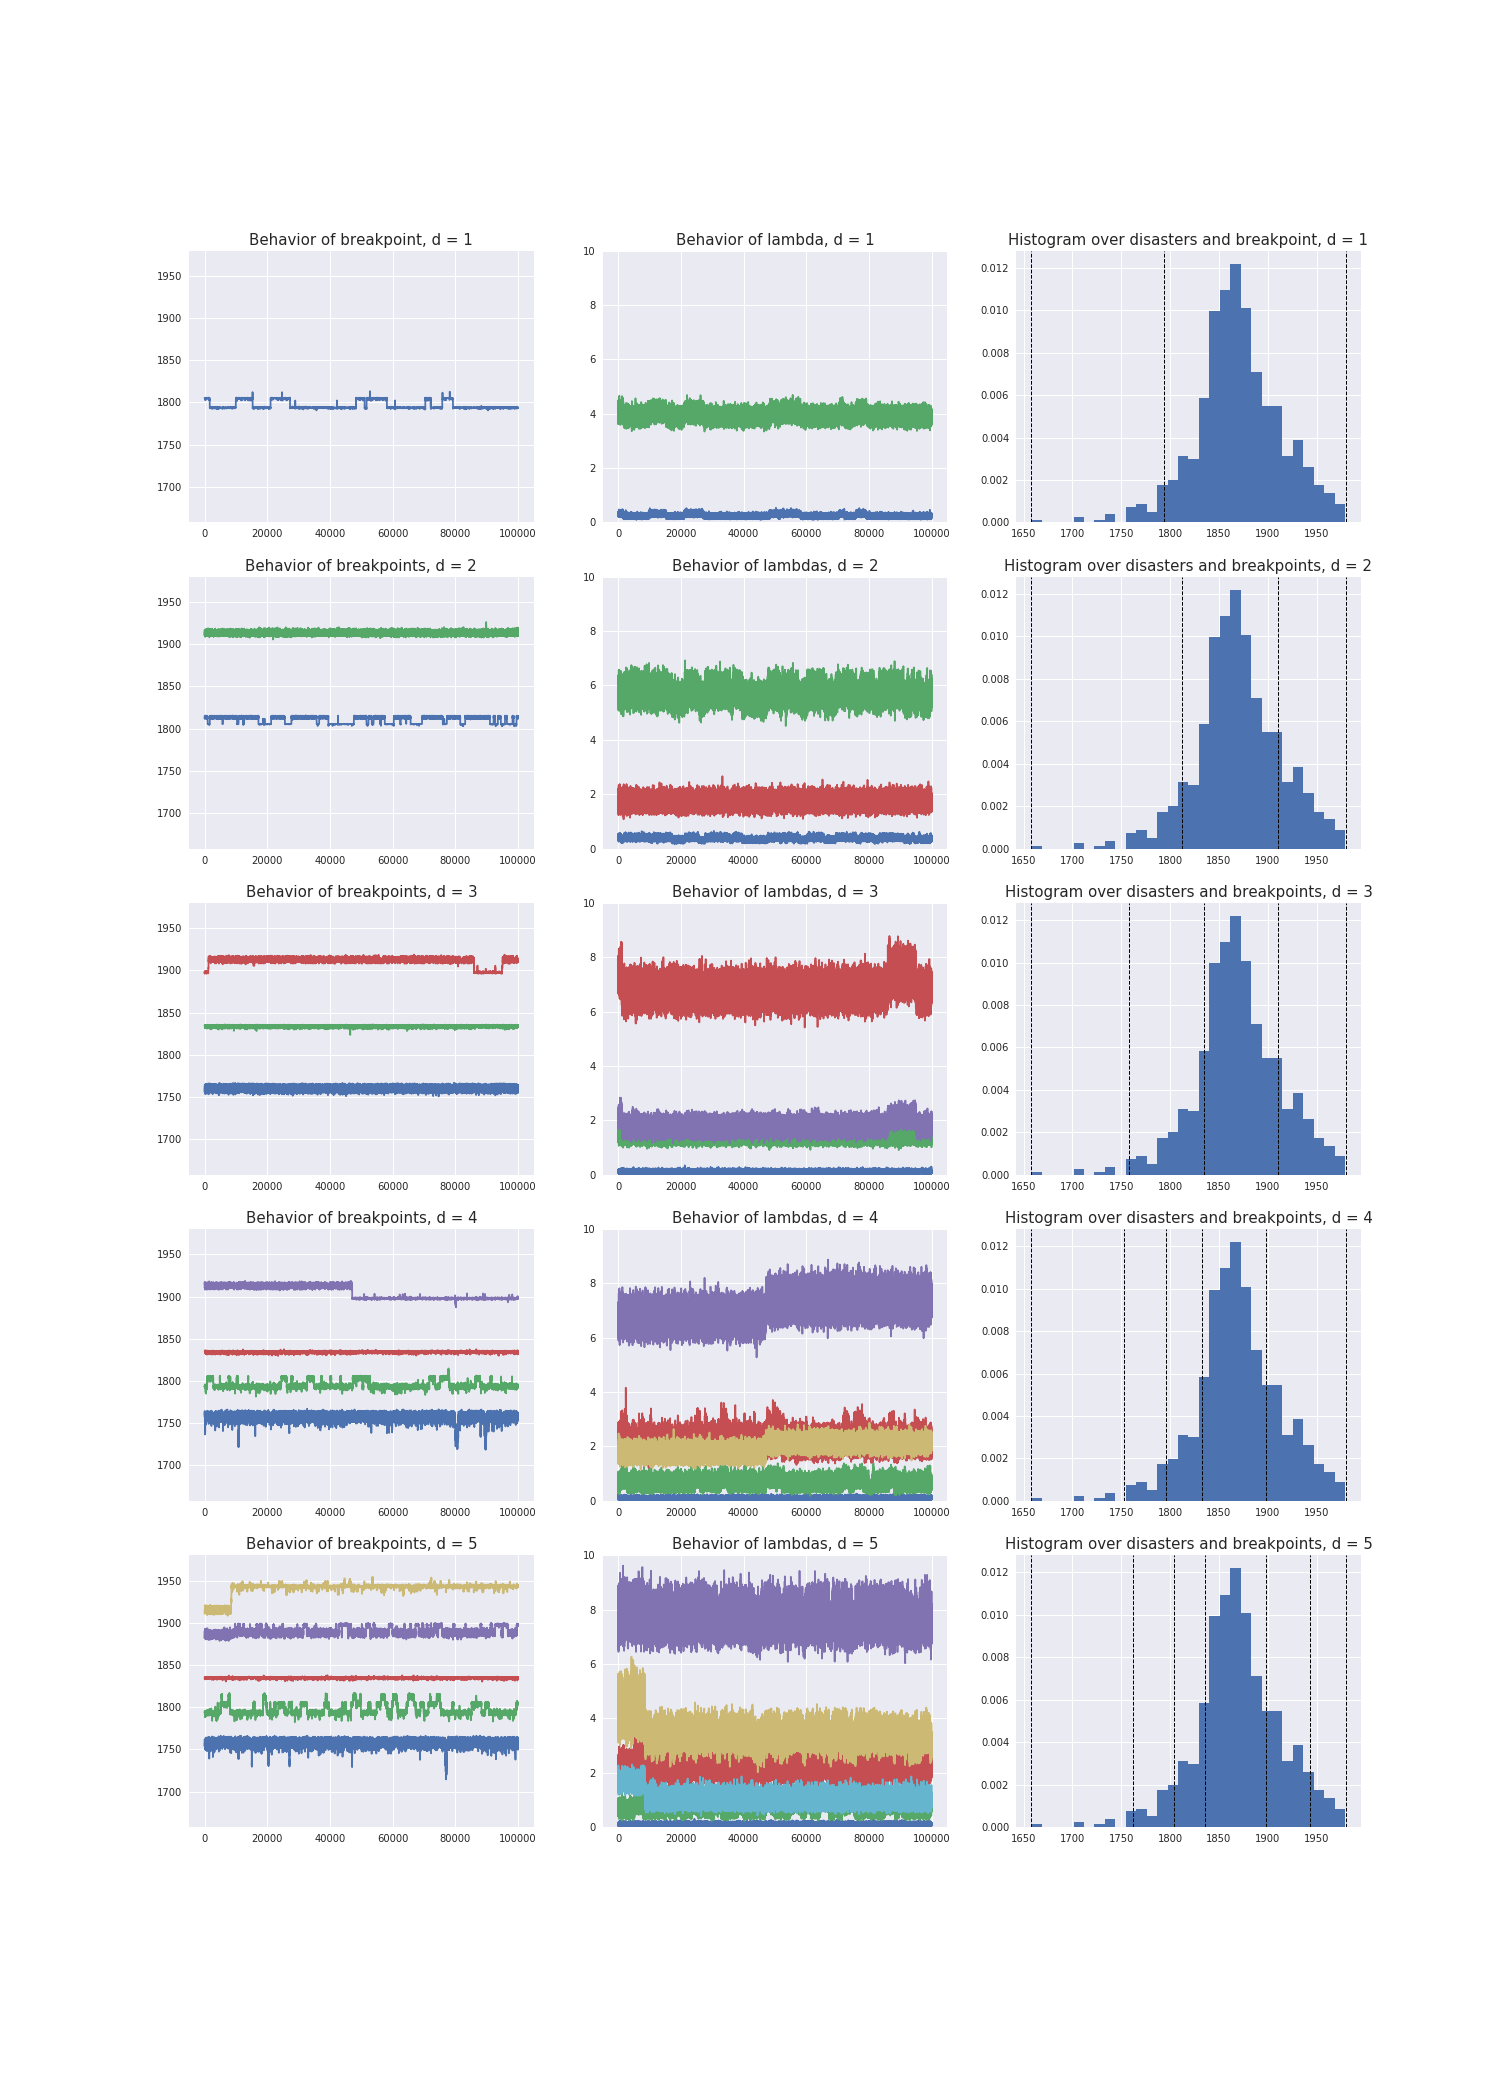
\includegraphics[width = 1.0\textwidth]{images/chain_behavior.png} 
    \caption{}
    \label{}
\end{figure}

\subsection*{2)}

To sample from $f(\lambda, \theta, t | \tau)$ we need to construct a hybrid MCMC sampler using both the Gibbs sampler and the Metropolis-Hastings algorithm. We begin by sampling a random number $\theta$ from its prior distribution, and then sample the random vector \textbf{$\lambda$} from its prior distribution depending on $\theta$. We also create breakpoints $t$ spaced evenly in the interval [1658, 1980]. Then the algorithm loops through following steps:
\begin{enumerate}
    \item Sample $\theta_{k+1}$ from $f(\theta|\tau, \lambda_k, t_k)$
    \item Sample $\lambda_{k+1}$ from $f(\lambda|\tau, \theta_{k+1}, t_k)$
    \item Propose $t_{k+1}$ from a random walk proposal
    \item Accept or reject $t_{k+1}$
\end{enumerate}

Here we use a random walk proposal for the breakpoints $t$.

\newpage

\section{Parametric bootstrap for the 100-year Atlantic wave}

\subsection*{a)}

The Gumbal distribution has the following cumulative distribution function

\begin{equation}
    F(x; \mu, \beta) = \exp\left(-\exp\left(-\frac{x-\mu}{\beta}\right)\right), \quad x \in \mathbb{R}
    \label{eq:gumbel}
\end{equation}

The inverse of (\ref{eq:gumbel}) is calculated as below

\begin{equation}
    F^{-1}(u; \mu, \beta) = \mu - \beta*\ln(-\ln(u))
    \label{eq:inv_gumbel}
\end{equation}

\subsection*{b)}

To calculate the parametric bootstraped 95\% confidence interval for the parameters the following steps was taken:

\begin{itemize}
    \item The historical data was loaded from the provided text file.
    \item Parameters, $\mu$ and $\beta$, was estimated with help of est\_gumbel.m.
    \item $10^5$ series, each containing 568 samples each, was generated with the help of (\ref{eq:inv_gumbel}).
    \item For each serie, new parameters was estimated and 95\% confidence intervall was calculated by looking at the quantiles.
\end{itemize}

The resulting confidence intervall for the parameters can be seen in table \ref{tab:parameters}.

\begin{table}[H]
    \centering
    \caption{Estimated parameters with 95\% bootstrapped confidence intervals.}
    \label{tab:parameters}
    \begin{tabular}{lrrr}
\toprule
Parameter &  Estimate &  95\% Upper bound &  95\% Lower bound \\
\midrule
  $\beta$ &     1.486 &             1.579 &             1.390 \\
    $\mu$ &     4.148 &             4.277 &             4.022 \\
\bottomrule
\end{tabular}

\end{table}

\subsection*{c)}

To calculate the one sided parametric bootstrapped 95\% confidence interval for the 100-year return value the following steps was taken:

\begin{itemize}
    \item $10^5$ sets of parameters was generated in the same way as in task a).
    \item $F(1-1/T; \mu, \beta)$ was calculated for each set of parameters, were $T = 3*14*100$.
    \item The one-sided upper quantile was calculated.
\end{itemize}

\begin{table}[H]
    \centering
    \caption{Estimated mean of the 100-year way and bootstrapped one sided 95\% confidence interaval}
    \label{tab:bigwave}
    \begin{tabular}{lrr}
\toprule
     Parameter &    Mean &  95\% Upper bound \\
\midrule
 100-year wave &  16.527 &            17.235 \\
\bottomrule
\end{tabular}

\end{table}

\begin{figure}[H]
    \centering
    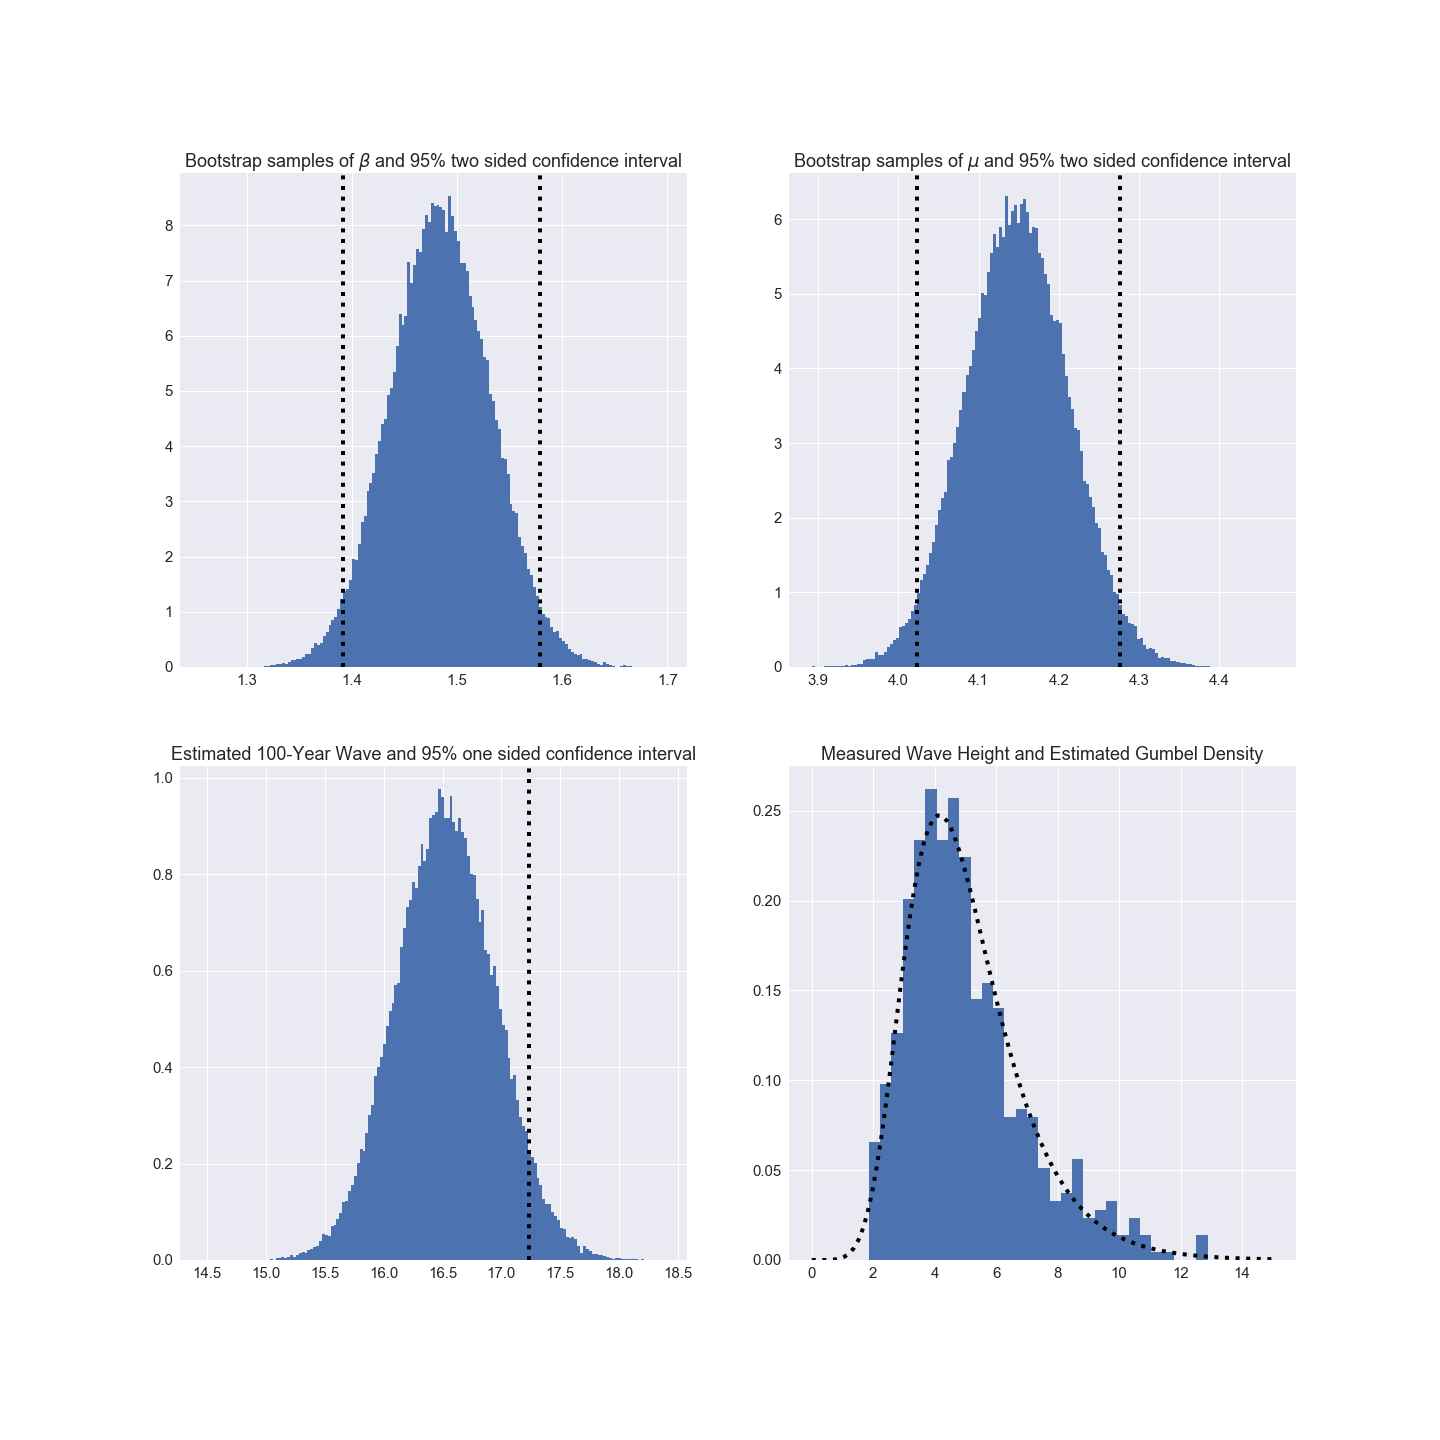
\includegraphics[width = 1.0\textwidth]{images/results_bootstrap.png}
    \caption{Densities over bootstraped parameters $\beta$ and $\mu$, }
    \label{}
\end{figure}

The resulting one-sided 95\% confidence interval for the 100-year wave is 17.24 m. The reason that we are interested in the upper quantile is that we want to get the worst scenario, by doing this, it's possible to say that the 100-year wave will with 95\% probability not be greater than 17.24 m. 

\end{document}